\documentclass[12pt,fleqn]{exam}
\usepackage{pifont}
\usepackage{dingbat}
\usepackage{amsmath,amssymb}
\usepackage{epsfig}
\usepackage{upgreek}
\usepackage[super]{nth}
\usepackage[colorlinks=true,linkcolor=black,anchorcolor=black,citecolor=black,filecolor=black,menucolor=black,runcolor=black,urlcolor=black]{hyperref}
\usepackage[letterpaper, margin=0.75in]{geometry}
\addpoints
\boxedpoints
\pointsinmargin
\pointname{pts}

\usepackage[activate={true,nocompatibility},final,tracking=true,kerning=true,factor=1100,stretch=10,shrink=10]{microtype}
\usepackage[american]{babel}
%\usepackage[T1]{fontenc}
\usepackage{fourier}
\usepackage{isomath}
\usepackage{upgreek,amsmath}
\usepackage{amssymb}
\usepackage{graphicx}

\newcommand{\dotprod}{\, {\scriptzcriptztyle
    \stackrel{\bullet}{{}}}\,}

\newcommand{\reals}{\mathbf{R}}
\newcommand{\lub}{\mathrm{lub}} 
\newcommand{\glb}{\mathrm{glb}} 
\newcommand{\complex}{\mathbf{C}}
\newcommand{\dom}{\mbox{dom}}
\newcommand{\range}{\mbox{range}}
\newcommand{\cover}{{\mathcal C}}
\newcommand{\integers}{\mathbf{Z}}
\newcommand{\vi}{\, \mathbf{i}}
\newcommand{\vj}{\, \mathbf{j}}
\newcommand{\vk}{\, \mathbf{k}}
\newcommand{\bi}{\, \mathbf{i}}
\newcommand{\bj}{\, \mathbf{j}}
\newcommand{\bk}{\, \mathbf{k}}
\DeclareMathOperator{\Arg}{\mathrm{Arg}}
\DeclareMathOperator{\Ln}{\mathrm{Ln}}
\newcommand{\imag}{\, \mathrm{i}}

\usepackage{graphicx}
\usepackage{color}
\shadedsolutions
\definecolor{SolutionColor}{rgb}{0.8,0.9,1}
\newcommand\AM{\textsc{am}}
\newcommand\PM{\textsc{pm}}
     
\newcommand{\quiz}{3}
\newcommand{\term}{Fall}
\newcommand{\due}{Wednesday 7 September 13:15 \PM}
\newcommand{\class}{MATH 115}
\begin{document}
\large
\vspace{0.1in}
\noindent\makebox[3.0truein][l]{\textbf{\class}}
\textbf{Name:} \hrulefill \\
\noindent \makebox[3.0truein][l]{\textbf{In class work \quiz, \term \/ \the\year}}
\textbf{Row and Seat}:\hrulefill\\
\vspace{0.1in}


\noindent  In class work  \quiz\/  has questions 1 through  \numquestions \/ with a total of  \numpoints\/  points.   
Turn in your work at the end of class  \emph{on paper}. This assignment is due \emph{\due}.

\vspace{0.1in}


\begin{questions} 

\question Find each of the following limits. Justify each of your 
steps by referencing one of our rules numbered zero through seven.

\begin{parts}
  
    \part[2] \(\displaystyle \lim_{x \to \uppi} \left(x^3 + x \right) \)
    \begin{solution}[1.5in]
        
    \end{solution}
      
    \part[2] \(\displaystyle  \lim_{x \to \sqrt{2}} \sqrt{x+1} \)
    \begin{solution}[1.5in]
        
    \end{solution}

    \part[2] \(\displaystyle  \lim_{x \to \sqrt{2}} \frac{x+1}{x-1} \)
    \begin{solution}[1.5in]
        
    \end{solution}

    \part[2] \(\displaystyle  \lim_{x \to 35} \sqrt{12 -2 \sqrt{x}} \)
    \begin{solution}[1.5in]
        
    \end{solution}


\end{parts}

%\newpage

\question A graph of a function $Q$ is shown. Using the graph,
as best you can find the numerical value of each limit.

\begin{parts}
    \part [1] \(\displaystyle \lim_{x \to 2} Q(x) \)
    \begin{solution}[1.5in]
        
    \end{solution}
    \part [1] \(\displaystyle \lim_{x \to -1^{(+)}} Q(x) \)
    \begin{solution}[1.5in]
        
    \end{solution}

\end{parts}

\begin{center}
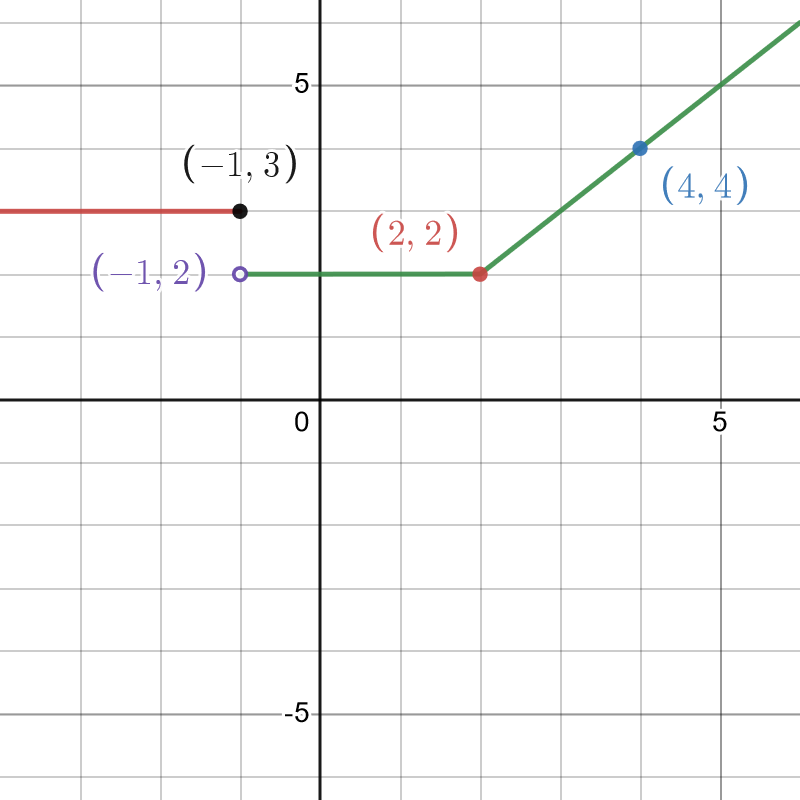
\includegraphics[scale=0.25]{desmos-graph(28).png}
\end{center}

\end{questions}

\newpage
\noindent Suppose functions $F$ and $G$ have limits toward $c$ and suppose $a,b \in \reals$ and $n$ is a positive integer. Then

\begin{description}

\item[Rule \#0 (constant)] $  \displaystyle \lim_{x \to c} (a) = a$.
 
\item[Rule \#1 (linearity)] $ \displaystyle \lim_{x \to c} (a F(x) + b G(x)) = a  \, \lim_{x \to c} (F(x)) + b \, \lim_{x \to c} (G(x)) $.

\item [Rule \#2 (product)]$ \displaystyle \lim_{x \to c} (F(x)  G(x)) = \, \lim_{x \to c} (F(x))  \times \lim_{x \to c} (G(x)) $.

\item [Rule \#3 (quotient)] Provided $\displaystyle  \lim_{x \to c} (G(x)) \neq 0$, we have $\displaystyle \lim_{x \to c} \frac{F(x)}{G(x)} = \, \frac{\lim_{x \to c} (F(x))}{ \lim_{x \to c} (G(x)) } $.

\item [Rule \#4 (power)]  $ \displaystyle \lim_{x \to c} F(x)^n  = \left(\lim_{x \to c} F(x) \right)^n  $.

\item [Rule \#5 (root)]  Provided $ \displaystyle  \left(\lim_{x \to c} F(x) \right)^{1/n} $ is real,  $ \displaystyle \lim_{x \to c} F(x)^{1/n}  = \left(\lim_{x \to c} F(x) \right)^{1/n}  $.

\item [Rule \#6 (polynomial)]  Provided $F$ is a polynomial, we have  $ \displaystyle \lim_{x \to c} F(x) = F(c)$

 \item [Rule \#7 (rational)]  Provided $F$ is a rational function and $c \in \dom(F)$, we have  \mbox{$ \displaystyle \lim_{x \to c} F(x) = F(c)$.}
\end{description}
\end{document}